%---------------------------------------------------
%	PACKAGES AND OTHER DOCUMENT CONFIGURATIONS
%------------------------------------------------------------------------------------


\documentclass[1 pt]{article}
\usepackage{amsmath,amsthm,amssymb}
\usepackage{mathtext}
\usepackage[T1,T2A]{fontenc}
\usepackage[utf8]{inputenc}
\usepackage[english,russian]{babel}
\usepackage{graphicx}
\usepackage{natbib}
\usepackage{pgfplots}
\usepackage[inkscapeformat=png]{svg}
\pgfplotsset{compat=1.9}

\begin {document}

\begin{titlepage}
\newcommand{\HRule}{\rule{\linewidth}{0.3 mm}} % Defines a Hnew command for the horizontal lines, change thickness here

\center % Center everything on the page
 
%----------------------------------------------------------------------------------------
%	HEADING SECTIONS
%----------------------------------------------------------------------------------------

\textsc{\Large Московский физико-технический институт }\\[1.5cm] % Name of your university/college
\textsc{\Large Факультет аэрокосмических технологий}\\[0.5cm] % Major heading such as course name
\textsc{\large Кафедра общей физики}\\[0.5cm] % Minor heading such as course title

%----------------------------------------------------------------------------------------
%	TITLE SECTION
%----------------------------------------------------------------------------------------

\HRule \\[0.4cm]
{ \huge \bfseries Измерение вязкости воздуха по
течению в тонких трубках }\\[0.4cm] % Title of your document
\HRule \\[1.5cm]
 
%----------------------------------------------------------------------------------------
%	AUTHOR SECTION
%----------------------------------------------------------------------------------------

\begin{minipage}{0.4\textwidth}
\begin{flushleft} \large
\emph{Автор:}\\ Артем \textsc{Овчинников} % Your name
\end{flushleft}
\end{minipage}
\begin{minipage}{0.4\textwidth}
\begin{flushright} \large
\emph{Преподаватель:} \\
Арина Владимировна \textsc{Радивон} % Supervisor's Name
\end{flushright}
\end{minipage}\\[4cm]
%	DATE SECTION
%----------------------------------------------------------------------------------------

{\large \today}\\[2cm] % Date, change the \today to a set date if you want to be precise

%----------------------------------------------------------------------------------------
%	LOGO SECTION
%----------------------------------------------------------------------------------------

 
%----------------------------------------------------------------------------------------

\vfill % Fill the rest of the page with whitespace

\end{titlepage}
\tableofcontents
\newpage
\section{Аннотация}
В данной работе представлено экспериментальное определение вязкости воздуха методом, основанным на
формуле Пуазейля.
\section{Теоретические сведения}
\begin{equation}
    Re = \frac{\rho u a}{\eta}
\end{equation}
- число Рейнольдса методом размерностей, где $\rho$ - плотность, $u$ - средняя скорость, $a$ - характерный размер (радиус), $\eta$ - вязкость.
\begin{equation}
    Q = \frac{\pi R^4 \Delta P}{8 \eta l}
\end{equation}
- формула Пуазейля.
\begin{equation}
    Q = const \cdot R^{5/2} \sqrt{\frac{\Delta P}{\rho l}}
\end{equation}
- формула объемного расхода для турбулентного потока
\section{Методика измерений}

\section{Используемое оборудование}
\begin{center}
    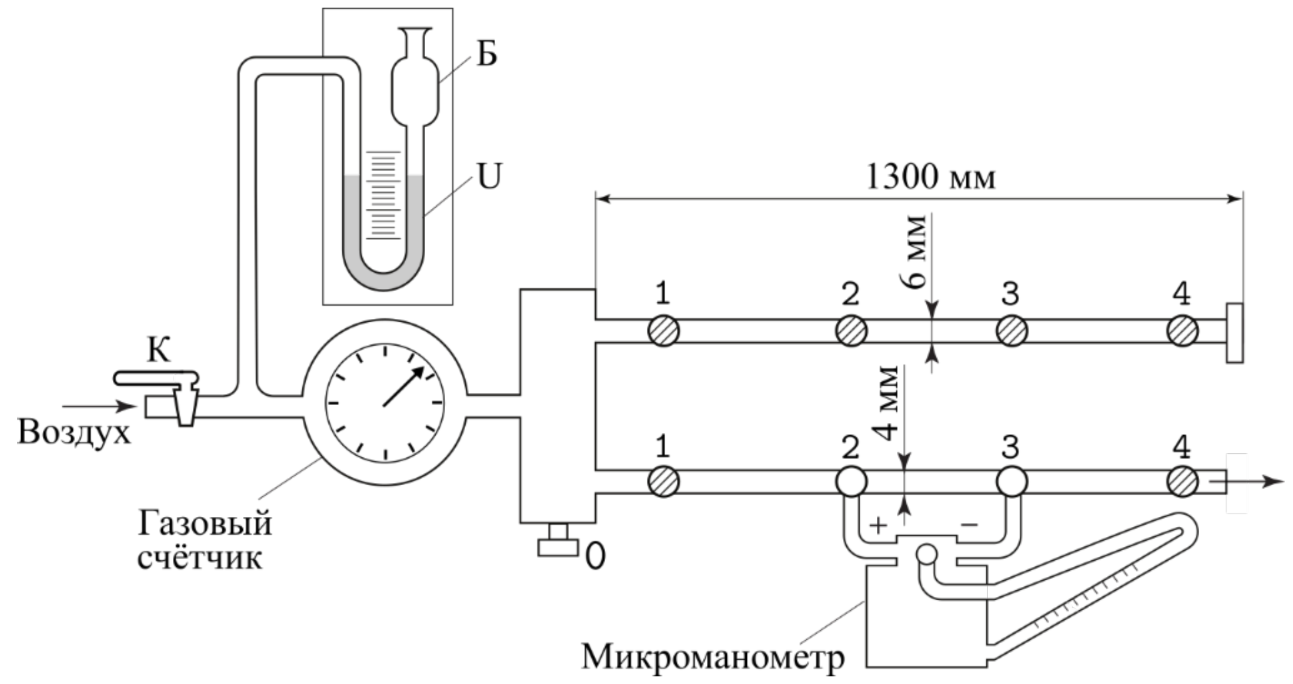
\includegraphics[scale=0.3]{physlabwork_5week_setup.png}
\end{center}

\newpage
\section{Результаты измерений и обработка данных}
\begin{center}
    \includesvg[]{physlabwork_5week_plot}
\end{center}
\begin{center}
    \includesvg[]{physlabwork_5week_plot_3}
\end{center}
\begin{center}
    \includesvg[]{physlabwork_5week_plot_2}
\end{center}
\begin{center}
    \includesvg[]{physlabwork_5week_plot_4}
\end{center}
\begin{center}
    \includesvg[]{physlabwork_5week_plot_5}
\end{center}
\section{Обсуждение результатов}
\section{Заключение}
\end{document}
